\documentclass[11.5pt, oneside]{article}   	% use "amsart" instead of "article" for AMSLaTeX format
\usepackage{geometry}                		% See geometry.pdf to learn the layout options. There are lots.
\geometry{letterpaper}                   		% ... or a4paper or a5paper or ... 
\geometry{legalpaper, portrait, margin=1in}
\usepackage[parfill]{parskip}    			% Activate to begin paragraphs with an empty line rather than an indent
\usepackage{graphicx}				% Use pdf, png, jpg, or eps§ with pdflatex; use eps in DVI mode
\usepackage{amssymb}
\usepackage{multicol}
\usepackage{abstract} 
\usepackage{graphicx}
\usepackage{caption}

\title{Saito: A Big-Data Blockchain with Proof-of-Transactions}
\author{David Lancashire}
\date{September 26, 2018\\v. 2.2.0}
\begin{document}
\maketitle


\begin{onecolabstract}
Saito is a blockchain designed to process terabytes of data every day, a level of scalability achieved by coupling a transient ledger to a proof-of-transactions mechanism that pays explicitly for the bandwidth and storage needed by the network. Saito continually evolves towards an optimal network structure while eliminating sibyl-attacks, fee-recycling attacks, block-withholding attacks and more. It provides a decentralized and efficient platform on which to build bandwidth-intensive Internet applications like email, social networks, cryptocurrency payment channels, and much more.
\end{onecolabstract}


\begin{multicols}{2}
Saito is a cryptocurrency designed for applications that need to send large amounts of data across the Internet. It can be used to build decentralized versions of most Google services, along with un-astroturfable Internet forums, social networks, pay-to-play websites, distributed key registries that are secure from MITM attacks, payment channels, and much more.

More generally, Saito can be considered a solution to the problem of how to build a terabyte-level blockchain. The design corrects all known collective action problems associated with existing consensus mechanisms, and permits scalability to the point that underlying network hardware rather than economic forces impose constraints on blocksize. We believe the practical limit for a Saito blockchain today is on the order of 100 TB of data per day, and advances in routing capacity will push us to the petabyte level within a decade.

If you are interested in the technical design of the Saito network, please skip to Section 2. In the next section we describe why a new consensus mechanism is needed to support big-data applications. This requires briefly explaining the underlying economic problems that frustrate scaling attempts as bandwidth and storage requirements grow, and what theoretical improvements are needed to overcome these design-imposed limitations.


1. THE PROBLEM

The problem with blockchain scaling is not at the network technology layer. At time of writing, data centres around the world are implementing 400 Gbps network switches while 100 Gbps connections are becoming standard even in lower-tier colocation facilities. If we had the resources to pay for the necessary equipment there is nothing technically stopping us from building a blockchain that is as decentralized as the public Internet backbone.

What limits network growth is the fact that no existing consensus mechanism pays directly for network operating costs. In the past, developers have waved away this limitation, claiming that as long as {\textit{someone}} is earning money from the network they will pay all costs needed to support it. Yet this is not the case, for while proof-of-work solved one collective action problem, it snuck two other collective action problems in through the back door: a tragedy-of-the-commons problem that results in an unsustainable and bloated blockchain, and a free-rider problem that leads to an underprovision of network routing. Neither problem is crippling at small scale, but both grow increasingly incapacitating as bandwidth and storage costs rise.

Fixing the tragedy-of-the-commons problem requires eliminating the permanent ledger, whose structure allows nodes to accept payment today for work that can be offloaded to others tomorrow. The resulting incentives to maximize present-day revenues and disregard long-term support costs can lead to bloated blockchains that will eventually collapse and more subtly to transaction mispricing, as users can pay fees that do not reflect the true cost of long-term storage on the blockchain. The fact that this is a fundamental problem is self-evident from the way Satoshi's solution is "not to care," yet while indifference may work on networks with low levels of non-mining costs, it stops being viable in environments that push the technical limits of network capacity and where bandwidth and storage costs constitute a non-trivial share of network expenditures.

Eliminating the tragedy-of-the-commons problem requires that all nodes which collect fees in exchange for processing transactions must fully bear the cost of processing those transactions for as long as they remain on the blockchain. In practice this means we need a way to either eliminate blockchain creep or defer fee collection so that payments are meted-out over time as nodes continue to do the work for which the fee was originally paid. Our solution accomplishing this is described fully in Section 2.

The free-rider problem is more subtle. Because proof-of-work and proof-of-stake reward mining and staking activities exclusively, these two consensus mechanisms strictly punish nodes which spend funds to support the public network and incentivize nodes to "free-ride" on their more altruistic peers. Although it is often claimed that miners in a proof-of-work network will pay to operate the public network and freely share the transactions they source (as otherwise the network cannot earn money), the economic incentives in bitcoin-class systems strictly punish this behavior. If any major bitcoin miner is so foolish as to spend 80 percent of its revenue to support a terabyte-level public network, any miner that can get away with paying less will be more profitable, and gradually expand its market share by pouring the additional profits into purchases of additional hashpower.

In economics, the only reliable solution to the free rider problem is eliminating open access to the network in question and ensuring that only those who pay to support a public good receive the benefits from it, similar to the way that governments typically limit welfare benefits to those who pay taxes into the system. Most existing proposals on how to scale a blockchain are forced by the underlying economic issues that they cannot solve into this set of trade-offs: all proposals of which we are aware involve either handling over control of the public network to a private actor, or closing off open access to parts of the network layer by selecting a subset of nodes which are eligible to collect a network subsidy.

Strictly speaking, neither approach offers an acceptable trade-off for a cryptocurrency, as the open access properties of a blockchain network are necessary for its decentralization and censorship-resistance. The governance attacks which node-selection algorithms enable also enable significant and new attack vectors. Building a blockchain that can process the massive amounts of data required by Saito-scale applications thus requires a new and better consensus mechanism. Specifically, it requires that we end the practice of rewarding abstract and unrelated "work" like mining and staking and instead build our security function around the actual work we need the network to do (i.e. propagating transactions and blocks). Our solution accomplishing this is outlined in Section 3.

2. THE TRANSIENT BLOCKCHAIN

In the Saito network we make two changes to enable terabyte-level scaling. The first is embracing a "transient blockchain" that solves the tragedy-of-the-commons problem inherent in blockchain design, and the second is the use of a novel consensus mechanism that we call proof-of-transactions (a.k.a. proof-of-routing or proof-of-relay) that solves the free-rider problem. 

The principle behind the transient blockchain is simple: allow the nodes in the network to delete the oldest blocks in the ledger at predictable intervals ("genesis periods"). The length of the genesis period can be set dynamically if needed. At the extreme of a blockchain designed to handle global email traffic, it may be as short as 24 hours.

As such, the transient blockchain can be considered a form of pruning where the UTXO slips added to new blocks simply become unspendable after a certain number of blocks, with this limit enforced by the consensus rules of the blockchain: transactions spending outdated slips are invalid by default. With no need to maintain a permanent ledger our transient blockchain allows old transactions to be removed at roughly the same rate that new transactions are added, allowing the network to accurately price the true cost of including and propagating a transaction through the network.\footnote[1]{The most resilient parasite of an idea in the blockchain community is the rarely-challenged notion that blockchains require permanent ledgers. This is false -- the purpose of a consensus mechanism is to allow the network to reach consensus about which tokens being *added* to the network have value; there is no need to guarantee that the value of the token persists into perpetuity. The only requirement from an economic perspective is that token value must persist for long enough that network operators can liquidate or transfer the tokens so as to fund their own operations.}

Under this system, the burden of archiving the network history passes -- as it does in the consumer Internet -- from the routing nodes in the network to the servers and users that actually care about the data. And in cases where it is desirable for data to remain on-chain, it can simply be rebroadcast to the front of the chain with the appropriate fee to cover the next genesis period. The automatic rebroadcasting of expiring slips can even be enabled, if desired, through the consensus rules of the blockchain, enabling the network to provide permanent storage for whatever users genuinely need and are willing to pay the cost of on-chain storage.

Critics may note the security trade-off in this approach: new nodes joining the network become vulnerable to attack at their point of initial connection. Yet this is not a problem unique to Saito, as the security that syncing from the genesis block offers is largely illusory. How many Bitcoin users check that their software is syncing from the correct hash? And how many are aware of the myriad ways that even a software client that uses the proper hash can subvert the security of a blockchain? The reality is that in blockchain as most other digital fields, the security is ultimately provided not by a single hash but rather by the entire software package that implements the consensus logic and manages peer connections.

While the transient blockchain avoids the problem of the blockchain collapsing under its own weight at massive scale, and ensures space can be priced accurately even as storage times approach infinity, it does not pay for the costs imposed on the nodes in the peer-to-peer network by the large data requirements of the network. To solve this second problem a new security method is needed, one we call proof-of-transactions.

3. PROOF-OF-TRANSACTIONS

Under proof-of-transactions, any node can create a block at any time provided it pays a "burn fee" set by the network as the cost of doing so. This burn fee is set to a high level immediately after a block is produced and decreases gradually until it hits zero, at which point any node on the network may produce a block for free. The burn fee ensures that the node has done the work required of block producers: assembling blocks that pay transaction fees to the network. 

Importantly, to prevent all nodes in the network from simultaneously producing blocks, the credit used to pay the burn fee is not the total value of the transaction fees included in the block but the "usable value" of those fees, which drops as the number of hops each transaction has made across the network increases. Because the resources available to produce blocks increases as the volume of transactions grows, because users can regulate the depth that their transactions propagate (and thus the speed of their confirmation) by adjusting their fees, and because nodes generally issue blocks as soon as it becomes profitable for them to do so, the pace of block production in Saito ends up being determined by the overall volume of transaction fees in the network.

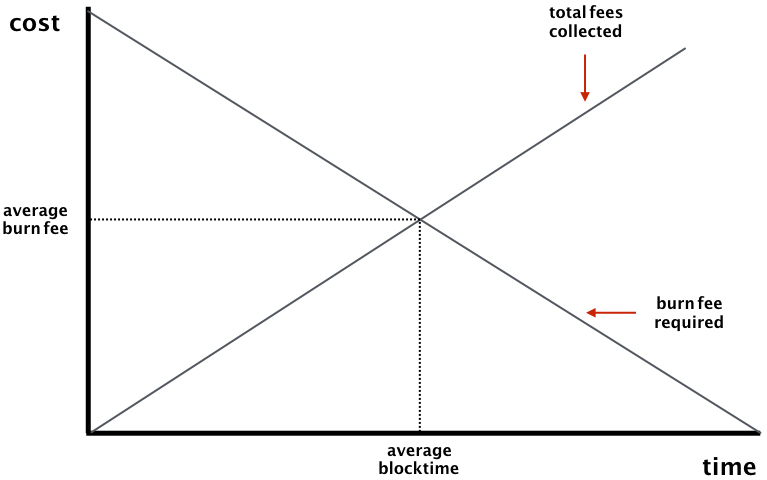
\includegraphics[width=.45\textwidth]{saito2.jpeg}

In practice, honest nodes route transactions and produce blocks for free while attackers must pay real fees to generate competing blocks. And conducting this sort of attack is expensive: as Figure 2 demonstrates it is impossible for attackers to produce blocks at a faster pace than the main chain without outspending the network as a whole.

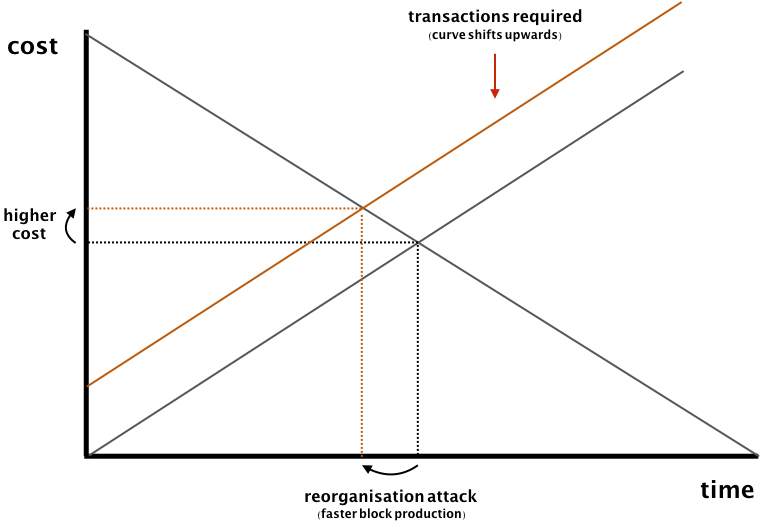
\includegraphics[width=.45\textwidth]{saito3.jpeg}

For reasons that are outlined in Section 4, Saito forces attackers to pay the entire burn fee rather than just cover the marginal difference over the amount required by the main chain. It also increases the cost of attacks over time by adjusting the burn fee upwards to keep blocktime constant as transaction volume grows. This enables Saito to offer comparable security to Bitcoin against chain-reorganization attacks in the sense that the cost of a chain-reorganization can always be quantified, and users that require significant guarantees against non-reversibility can calculate the expense and wait the appropriate number of confirmations.

There is a major problem with this approach however, which lies in the economic consequences of requiring nodes to burn capital to produce blocks:

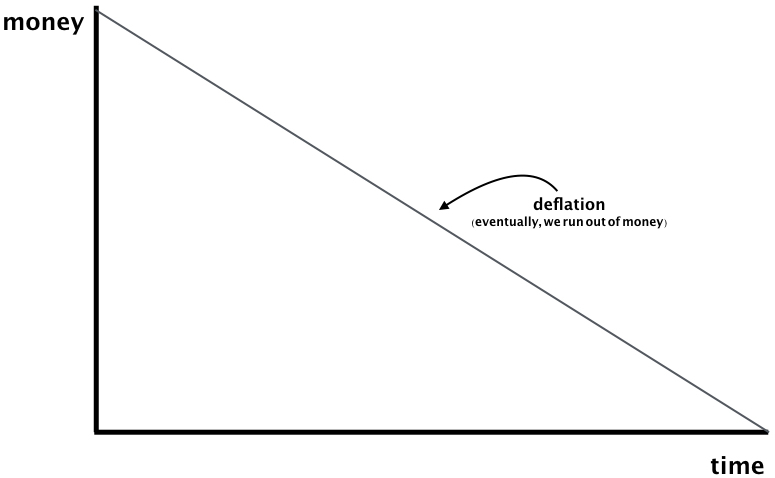
\includegraphics[width=.45\textwidth]{saito4.jpeg}

Avoiding a deflationary crash requires us to inject tokens into our network. But how can we do this? Saito cannot follow in the footsteps of Bitcoin and hand over the fees included in the block directly to the block producer as a form of payment. Doing so would eliminate the entire point of having a burn fee by enabling fee-recycling attacks on the network. Splitting the available funds between various nodes in the network would be a better option, but even then how can one fairly select winners? The network cannot use any variable associated with the block itself for this purpose, since as long as the block-producing node has any influence over how funds are allocated a savvy attacker can sibyl the network for profit and/or simply focus on gaming the token-issuing mechanism, reducing the security mechanism to a thinly-disguised proof-of-work.

Fortunately, there is a solution to this problem, which involves recycling the burned tokens back into the network through a process that cannot be co-opted by any of the players in the network. We achieve this through a zero-sum competition between bandwidth-expending nodes and CPU-expending miners in the network. We call this battle for the "paysplit" of the network.

4. PAYSPLIT

Whenever a node produces a block, it collects what profit it can (the difference between the value of usable fees included in the block minus the necessary burn fee) and bundles all remaining fees into a "golden ticket" that contains (1) a computational puzzle for miners to solve, and (2) a vote to increase, decrease, or hold constant the "paysplit" of the network (the percentage of all golden tickets that are paid out to miners). By default, these tickets are included in all blocks produced. Miners listening on the network choose which blocks to solve and -- should they find a solution to the cryptographic puzzle -- propagate their solution back into the network as a regular fee-paying transaction. In addition to containing an independently verifiable proof-of-solution, these miner transactions also include a separate vote on whether to increase, decrease, or hold constant the difficulty of the computational puzzle.

The golden ticket system can be visualized as follows:

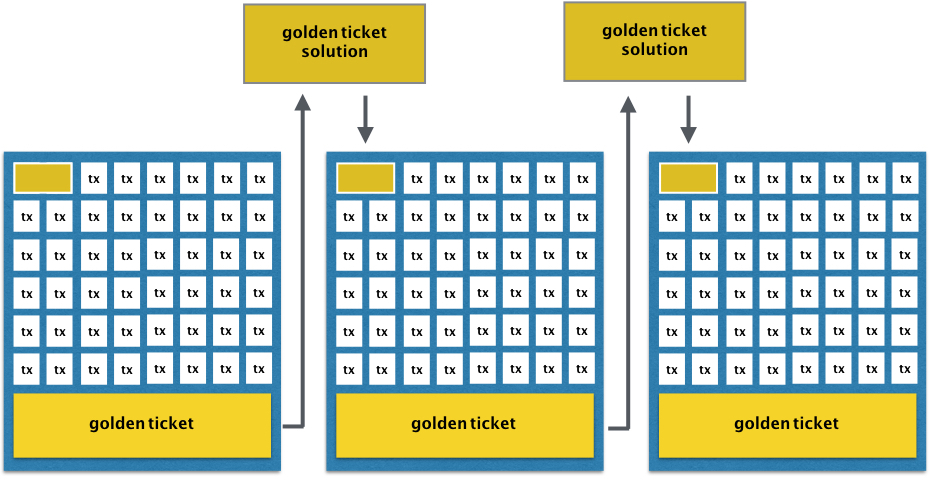
\includegraphics[width=.45\textwidth]{saito7.jpeg}

In order to increase the security of the blockchain, we specify that only one solution may be provided for any golden ticket, and that a solution must be included in the very next block to be considered valid. If these conditions are met, our two votes take effect, and the funds locked into the golden ticket are released to the network, split between the miner that found the solution and a random node in the peer-to-peer network. In the event a "golden ticket" is not solved, the funds are locked away and eventually fall off the transient blockchain, at which point they can be recycled back into our economy in the coinbase of another golden ticket. 

This game is counterintuitive to most blockchainers because it separates the act of "producing blocks" from the act of "distributing tokens". This puts all actors into a delicate dance requiring collusion and cooperation alike. While both nodes and miners want at least one solution per golden ticket (because otherwise no-one gets paid), their interests otherwise diverge: miners prefer a high paysplit and high difficulty level, while nodes prefer a low paysplit and low difficulty level. Given that votes must pass between both players to change consensus settings, we end up with a competitive dynamic where both groups are constantly trading-off their individual short-term against their collective long-term interests. Full-nodes that gain miner support will produce blocks at a faster rate and be more profitable than those which do not. It is the cost of bandwidth and security provision relative to their incomes which determine the optimal strategies of both routing nodes and miners alike.

There are many obvious variants, such as the replacement of the mining puzzle with a proof-of-stake variant. And there is a lite-version of Saito that does not include the voting mechanism at all -- paysplit can be hard-coded so that it can only be changed through a hard fork. Another design decision we believe improves on the method (and reinforces the bounded rationality of the system as a whole) is giving an optional paysplit vote to the originators of transactions on the network. Should a user originate a transaction containing such a vote, Saito's consensus rules insist that it can only be included in a block which votes in the same direction. Users who choose to take sides in the ongoing struggle between nodes and miners thus sacrifice the reliability and speed of transaction confirmation, but gain marginal influence over how the network allocates resources and manages its security trade-offs.

5. ADDITIONAL SECURITY

Saito takes additional steps to secure the network. In order to deter sybilling, Saito has nodes sign transactions as they propagate through the network, adding to each an unforgeable history of the path it takes from its point of origin to its point of confirmation.As mentioned above, each hop a transaction takes along the network decreases the amount of the transaction fee that nodes can allocate to paying burn fees, making it pointless for routing nodes to add additional paths and incentivizing nodes in the central network to actively improve the efficiency of the network routing layer. We also specify that nodes cannot use any transaction fees from transactions that do not include them in their transaction path in order to ensure that attackers cannot lower their cost of attack by stealing transactions from honest nodes. In order to ensure that nodes cannot influence the distribution of funds from the golden ticket, we also specify that the node in the peer-to-peer network which wins the node share of the golden ticket is selected using a random variable sourced from the miner solution, with the winner selected from the pool of nodes contained in the transaction propagation paths found in the previous block, weighted -- obviously -- according to the usable value of the transactions they processed.

These additional restrictions secure our network from common attacks in other cryptosystems which -- oddly -- are not commonly recognized as attacks. In Saito, for instance, transactions are naturally valuable to nodes which participate in the P2P network and useless to attackers who lurk on the edges. Fee-sourcing attacks and transaction theft are also impossible: the fact that nodes must participate in the P2P network to harvest transactions even defends us against subtle attacks like those posed by the bitcoin FIBRE network, a closed-access network which benefits its participants by undermining the profitability of nodes which support the peer-to-peer network. Sybilling becomes an unprofitable strategy because it adds hops in transaction routes, making sibyls visible to other nodes and providing an evolutionary mechanism whereby weaker nodes that permit themselves to be sybilled lose revenue over time and are forced off the network by economic pressures. 

And hoarding? While it is possible for nodes to hoard transactions, it is strongly disincentivized as even nodes that merely participate in transaction routing have a chance of winning the golden ticket reward. Over the mid-term, even nodes that do not produce blocks blocks at all are still rewarded in proportion to the value of the transactions they direct inwards from the outer edges of the network.

Security is also reinforced by the competitive economic structure of our game in fascinating ways. Note that if network security falls too low, the network is incentivized to increase it by voting to pay miners more. How this secures the network is worth consideration since there are multiple mechanisms in play. Not only does greater difficulty make it difficult for attackers to overpower the existing chain, but a higher paysplit also supports the threatened chain in the long-run, speeding up block-issuance as more miners are drawn into the network and compete to have their solutions included over those of their peers. And even in situations where the network is not under active attack, the miner/node battle over the paysplit also serves a defensive "canary in the coalmine" function, encouraging nodes and miners to issue their own pro-miner blocks and pro-node solutions if they control enough hashpower or bandwidth to support their preference.

6. SUMMARY

Saito is a solution for building a massively-scalable blockchain. We achieve this scalability not through algorithmic tweaks to existing technologies, but rather by solving the underlying economic problems that create distorted economic incentives in all existing blockchain designs.

Those who pour over the technical details of our consensus mechanism will find embedded in it at least seven major innovations in blockchain technology: the transient blockchain, the burn fee, the usable transaction fee, the golden ticket system, a secure multi-party voting mechanism enforced by economic competition, automatic transaction rebroadcasting, and the chain of cryptographic signatures with cascading value that permits our network to identify and reward productive nodes in the network.  

We are keen for people to start building on Saito and welcome contact from other blockchain projects looking to incorporate one or several of these methods in their own networks. We encourage everyone to visit our website (http://saito.tech) where we maintain a working demo of the network, a roadmap outlining our development plans, links to downloadable software, and tutorials that can help anyone get started building Saito applications *today*.

\end{multicols} 
\end{document}
